\chapter{Design}
The system's design is critical to understand the project and an important metric to measure the project's success. This section entails the design process of different system parts and the application's high-fidelity prototypes.

\section{Research behind the design}
The design of this web app was done keeping in mind the summary of the background research. To make sure the requirements set in the background research were met, further research was needed to fulfil these requirements.

\subsection{Questionnaire for applicants}
To ensure that the jobs shown on the job applicant's side match their requirements and what they are looking for in a role, they will be asked questions when signing up for this application. These questions will all be multiple-choice or tag-based, which will be less time-consuming for applicants and easier for them simultaneously. The time taken by these questions should ideally be lesser than three minutes. These questions would then help match the applicants to job applications. 

It is also essential to choose the right questions to ask the applicants and have certain restrictions on the questions having tags to prevent users from selecting many of them. The questions asked to applicants are based on the mix of questions an employer looks for in an employee and vice-versa. \parencite{Reference28}

Questions asked to users would be:
\begin{enumerate}
    \item \textbf{Which city would you like to work in?} This will include a remote option and top cities throughout the United Kingdom.
    \item \textbf{What role do you want to work in?} This question will be tag-based, with many answers an applicant can choose from. A follow-up question will be asked based on this option, in which the applicant will choose the role most relevant to them. For example, suppose an applicant selects Software Engineering. In that case, they will get multiple roles in Software Engineering like Back-end engineer, front-end engineer, DevOps Engineer, Game Engineer, etc., which they can choose from. This will make it easier for the application to match them with the relevant role. A restriction of a maximum of three positions will be put in place for this answer.
    \item \textbf{What level of a job are you looking for?} Multiple answers with a restriction of a maximum of two will be given for this question. Internships, Entry-level jobs, Senior-level jobs, etc., will be answers a user can select.
    \item \textbf{What  are your favourite technologies?} An applicant will be given a tag-based question where they can select the must-have technologies and nice-to-have technologies. 
    \item \textbf{What technologies do you not like?} Here, an applicant will be again given a tag-based question where they can select the technologies they don't want to use in their future role.
    \item \textbf{When can you start?} This will have multiple options, including: In the following year, As soon as possible, I just want to have a look, etc.
    \item \textbf{Minimum expected salary?} In this question, the applicant can enter the minimum salary they would be expecting for the roles they would apply for. 
    \item \textbf{Do you need a visa to work in the UK?} This will be a Yes or a No question. Jobs which do not sponsor applicants to work in the UK will be hidden or shown based on this answer.
\end{enumerate}

Similar questions will be asked of employers for each job they post on the platform. Employers must answer these questions, which will let the application match the employers to the applicants based on the job and the job applicant's requirements. 

\section{System Requirements}
A set of requirements for each component of the project are defined below to ensure the aims, objectives and design requirements of the project are met.

\subsection{Front-End Requirements}
To make the application appealing and eye-catching, the front end needs to look modern, only having necessary details and not overloaded with information.

To ensure that these conditions are met, the front end needs to have the \break following:
\begin{enumerate}
    \item An appealing website home page: The homepage should be able to grab the attention and create a first impression on the user as soon as they open it. 
    \item Optimised for mobile phones: Users should be able to open and use the website on their mobile phones.
    \item A login page for job applicants and employers to access specific website pages.
    \item Specific routes which require logging in should not be accessible to users not logged in.
    \item Allow users to log in and log out of the website.
    \item Allow easy navigation from web pages.
    \item Have an interactive design for users.
\end{enumerate}

\subsection{Back-End Requirements}
An algorithm is needed to match the data provided in each job to the applicant's requirements. This algorithm will be used in the back end, written in JavaScript.

The requirements for the back end of this application are:
\begin{enumerate}
    \item Match jobs with applicants using an algorithm which matches the job's requirements to the applicant's requirements.
    \item Efficiently read the data from the front end and output the necessary data to the user side.
    \item Write readable code for other developers to grasp quickly.
\end{enumerate}

\subsection{Database Requirements}
The database, MySQL in this case, will store information of all users, including different jobs, user information, etc. 

The database requirements for this application are:
\begin{enumerate}
    \item Store data of users securely in the database using algorithms like hashing to ensure the data is secure even through a data breach. \parencite{Reference29}
    \item The database should allow quick and easy data retrieval.
    \item Reduce redundancy in the database, leading to slow data retrieval and unnecessary information.
\end{enumerate}

\subsection{Functional Requirements}
The functional requirements of this application are needed to identify what the system should achieve for users to do their tasks and also to understand any limitations this application might have. Functional requirements, defined below, are the minimum standard for what the application should be able to do for users to achieve their tasks and use this web app efficiently.

The research done into creating an app such as this has resulted in the following functional requirements:
\begin{enumerate}
    \item This application should be able to run on different browsers and mobile phones as well.
    \item It should be able to store the user data on the database securely and allow users to log in and register for this web app.
    \item The application should stay logged in for a specific time if the user has not logged out, even if the user has closed the browser.
    \item The application should provide an interface of different jobs to applicants which they can choose from.
    \item The application should allow employers to register their companies and add jobs.
    \item The application should be able to send an automated email to users each time they apply for a job and when they register for a job. 
\end{enumerate}

\subsection{Non-Functional Requirements}
The non-functional requirements can be used to judge the operation of a system. These are as follows:
\begin{enumerate}
    \item The matching algorithm which matches the jobs to the applicants should not take longer than 5 seconds.
    \item Each page must load within 2 seconds.
    \item The system must meet Web Content Accessibility Guidelines. \parencite{Reference30}
    \item The application's interface has to be user-friendly and easy to use.
\end{enumerate}

\subsection{User Requirements}
The user requirements contain the basic things users should be able to do in the MVP. These are as follows:
\begin{enumerate}
    \item Job applicants should be able to see jobs that match their requirements
    \item Job applicants should be able to edit their answers to the "quiz" based on the change of requirements they have through their careers.
    \item Users should be able to log in and register, and a display message should pop up if a wrong password/username is given.
    \item Employers should be able to add a new job to the platform.
    \item Employers should be able to see the applicant's profile, including their resume and other data the applicant wants to share with them.
\end{enumerate}

\section{System Design}
This section consists of the database design, which will be used in this application to store data, Use Case diagrams which constitute different user journeys and some designs and wireframes for this application. 

\subsection{Database Design}
The database design is an essential component for this application to store and use the data provided by users in the web application. A good database design also makes locating information in the web app easier and is crucial in efficiently executing queries and ensuring information consistency. For these reasons, the database must be correctly designed to make it easier to locate information and reduce redundancy.

\subsubsection{Entity Relationship diagram}
An ERD is used to visualise the relationship between each table in the database. It is essential to design an ERD before creating it as it helps debug future bugs and identify any design flaws before and during the development stage. Each row in every table should also have the correct data type for each column in SQL to determine what kind of data is expected inside each column and to ensure that accurate information is stored inside each table.

The ERD created contains two main tables which have the user's information. This is the information that isn't changed often and isn't directly linked to the specification of a job. A job applicant's name, LinkedIn URI and Rèsumè/CV are a part of this table. This table can add multiple rows as the application grows, but this information is sufficient for the MVP. 

Similarly, for Employers, the data that doesn't frequently change, like the company logo or slogan, is part of the top-level table called employers. Under this table, different jobs are created, which can then be matched to the user requirements in the back end of the application. No direct relation is needed between applicants and employers as this will be done at the back end of the application.

The relationships of different tables are shown below:
\begin{enumerate}
    \item Applicant Information to Applicant Requirements: This is a one-to-one relationship as an applicant is only allowed one set of requirements. The jobs the applicant gets shown will be dependent on these requirements. The user id is the key used in both tables to identify each row uniquely.
    \item Employers to Jobs: This is a one-to-many relationship as one company can create several jobs, each having different specifications and other requirements. The company id is the key used in all job tables and employers, which helps to identify the company that has put out the job uniquely.
\end{enumerate}


\begin{figure}
    \noindent
    \centering
    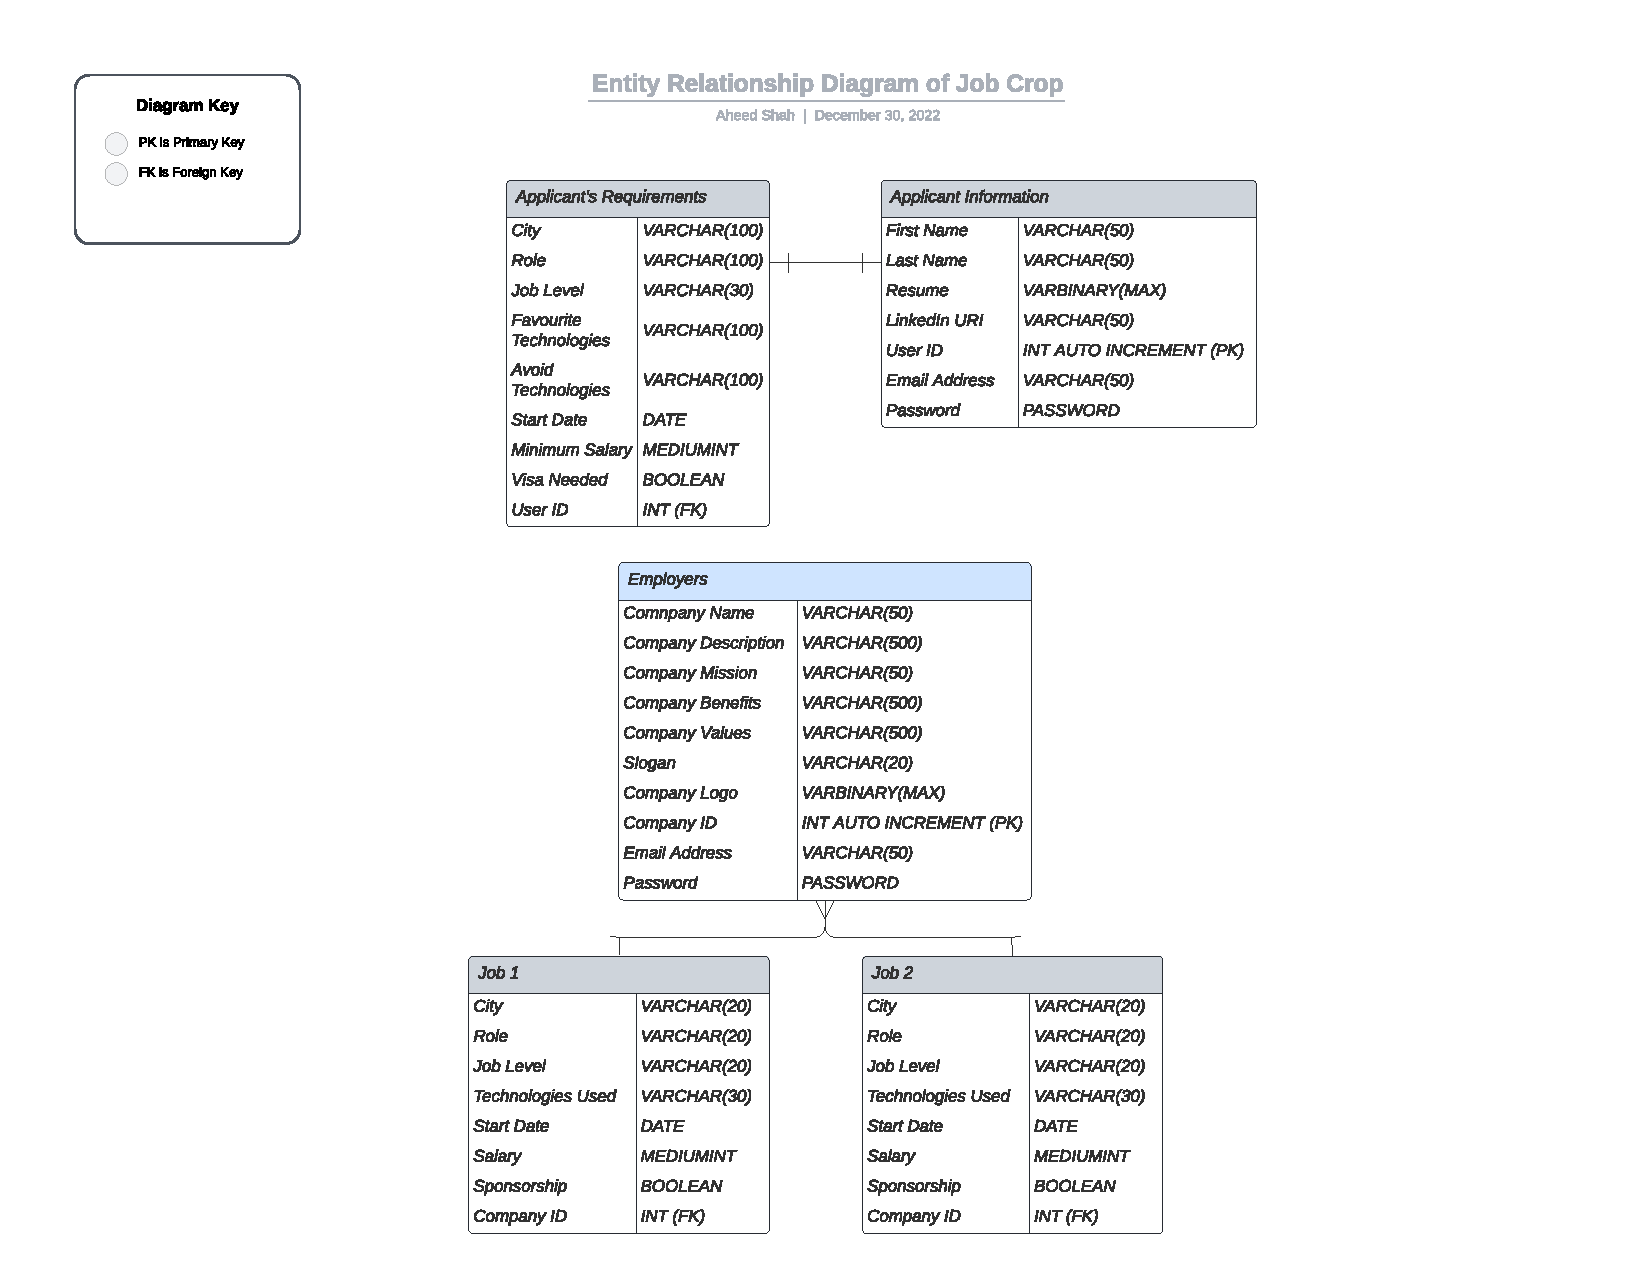
\includegraphics[width = 140mm]{Figures/ERD.pdf}
    \decoRule
    \caption[Entity Relationship Diagram]{Entity Relationship Diagram of the application}
    \label{fig: Entity Relationship Diagram}
\end{figure}

\subsection{Use Case Diagrams}
Use case diagrams specify the expected behaviour between the user and the application. These diagrams also help to visualise some of the different user journeys a user takes while using the application. 

Figure \ref{fig: Use Case Diagrams for Signing Up or Logging into the application} shows a user journey for a user to log in. If a user does not have an account with this application, they will be asked to sign up. Upon signing up and completing the questionnaire, they will be shown their specific matches based on these questions.

Figure \ref{fig: Use Case Diagram for applying for a job} shows a user journey for an applicant to apply for a job. It is similar to the previous user journey in the logging-in stage at first, but after the user gets shown different positions, they can apply for them or continue looking for another role. When they find the perfect role, they can click on the apply now button, which will allow them to continue to complete their application if there are any job-specific answers the employer needs the applicant to answer. As some jobs require users to go to specific companies' websites to apply, they can be redirected to that website to continue their application on a third-party website. The option to let users apply from this application, the company's own website, or both lies with the employer.

Figure \ref{fig: Use Case Diagram for an Employer to add a new job} shows a user journey of an employer adding a new job or looking through the applicants who have applied for the job posting. The use case diagram is quite similar in the login and sign-up stage, but employers get shown a different interface to look through the applicants for their previous job postings or the option to add a new job. To add a new job, an employer has to submit a similar questionnaire to what the applicant submits as their requirements. After this is successful, the job is added to the platform, and applicants can apply.

Creating these use case diagrams was quite helpful as the critical user workflows were thought about in detail when designing these workflows. It also helped outline the separate steps of different processes in sequential order. 

\begin{figure}
    \noindent
    \centering
    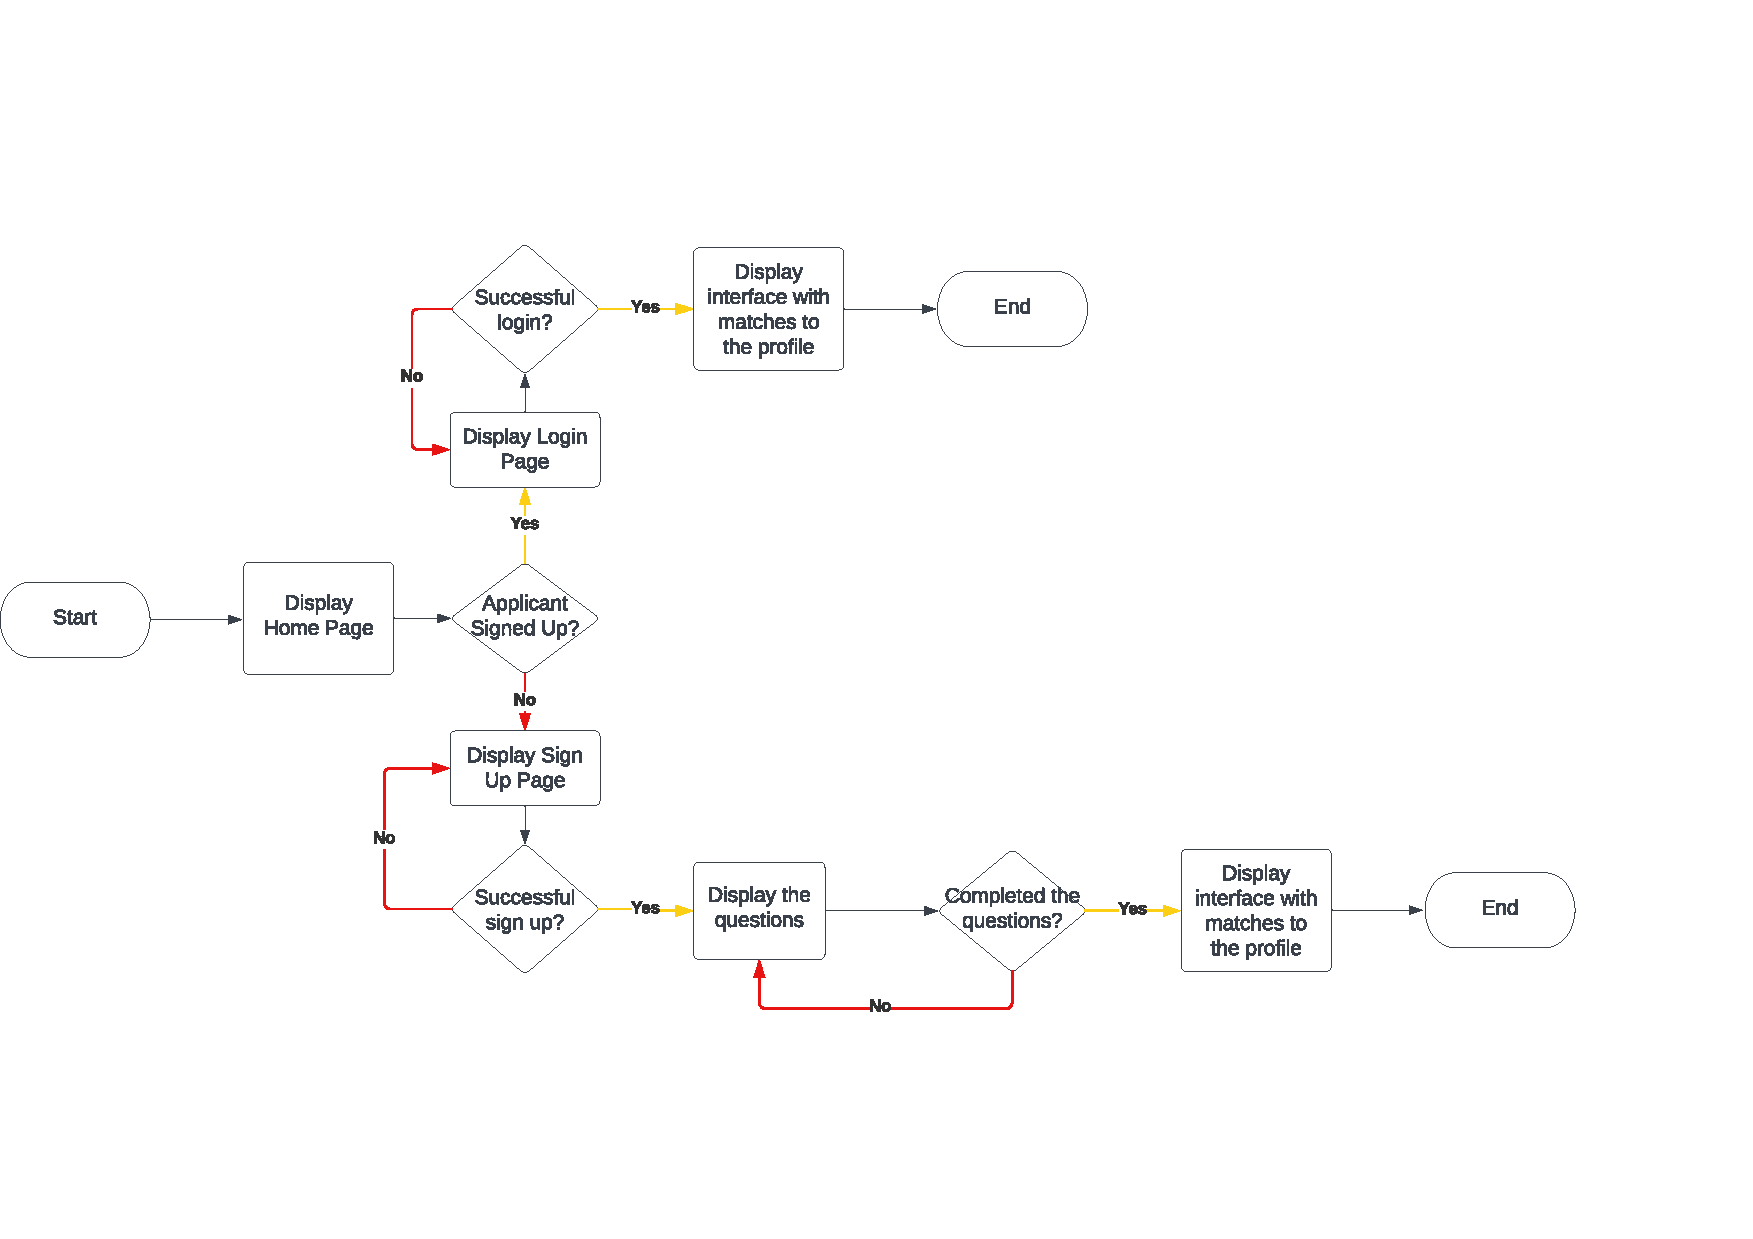
\includegraphics[width = 140mm]{Figures/signup.pdf}
    \decoRule
    \caption[Use Case Diagrams for Signing Up or Logging into the application]{Use Case Diagrams for Signing Up or Logging into the application}
    \label{fig: Use Case Diagrams for Signing Up or Logging into the application}
\end{figure}

\begin{figure}
    \noindent
    \centering
    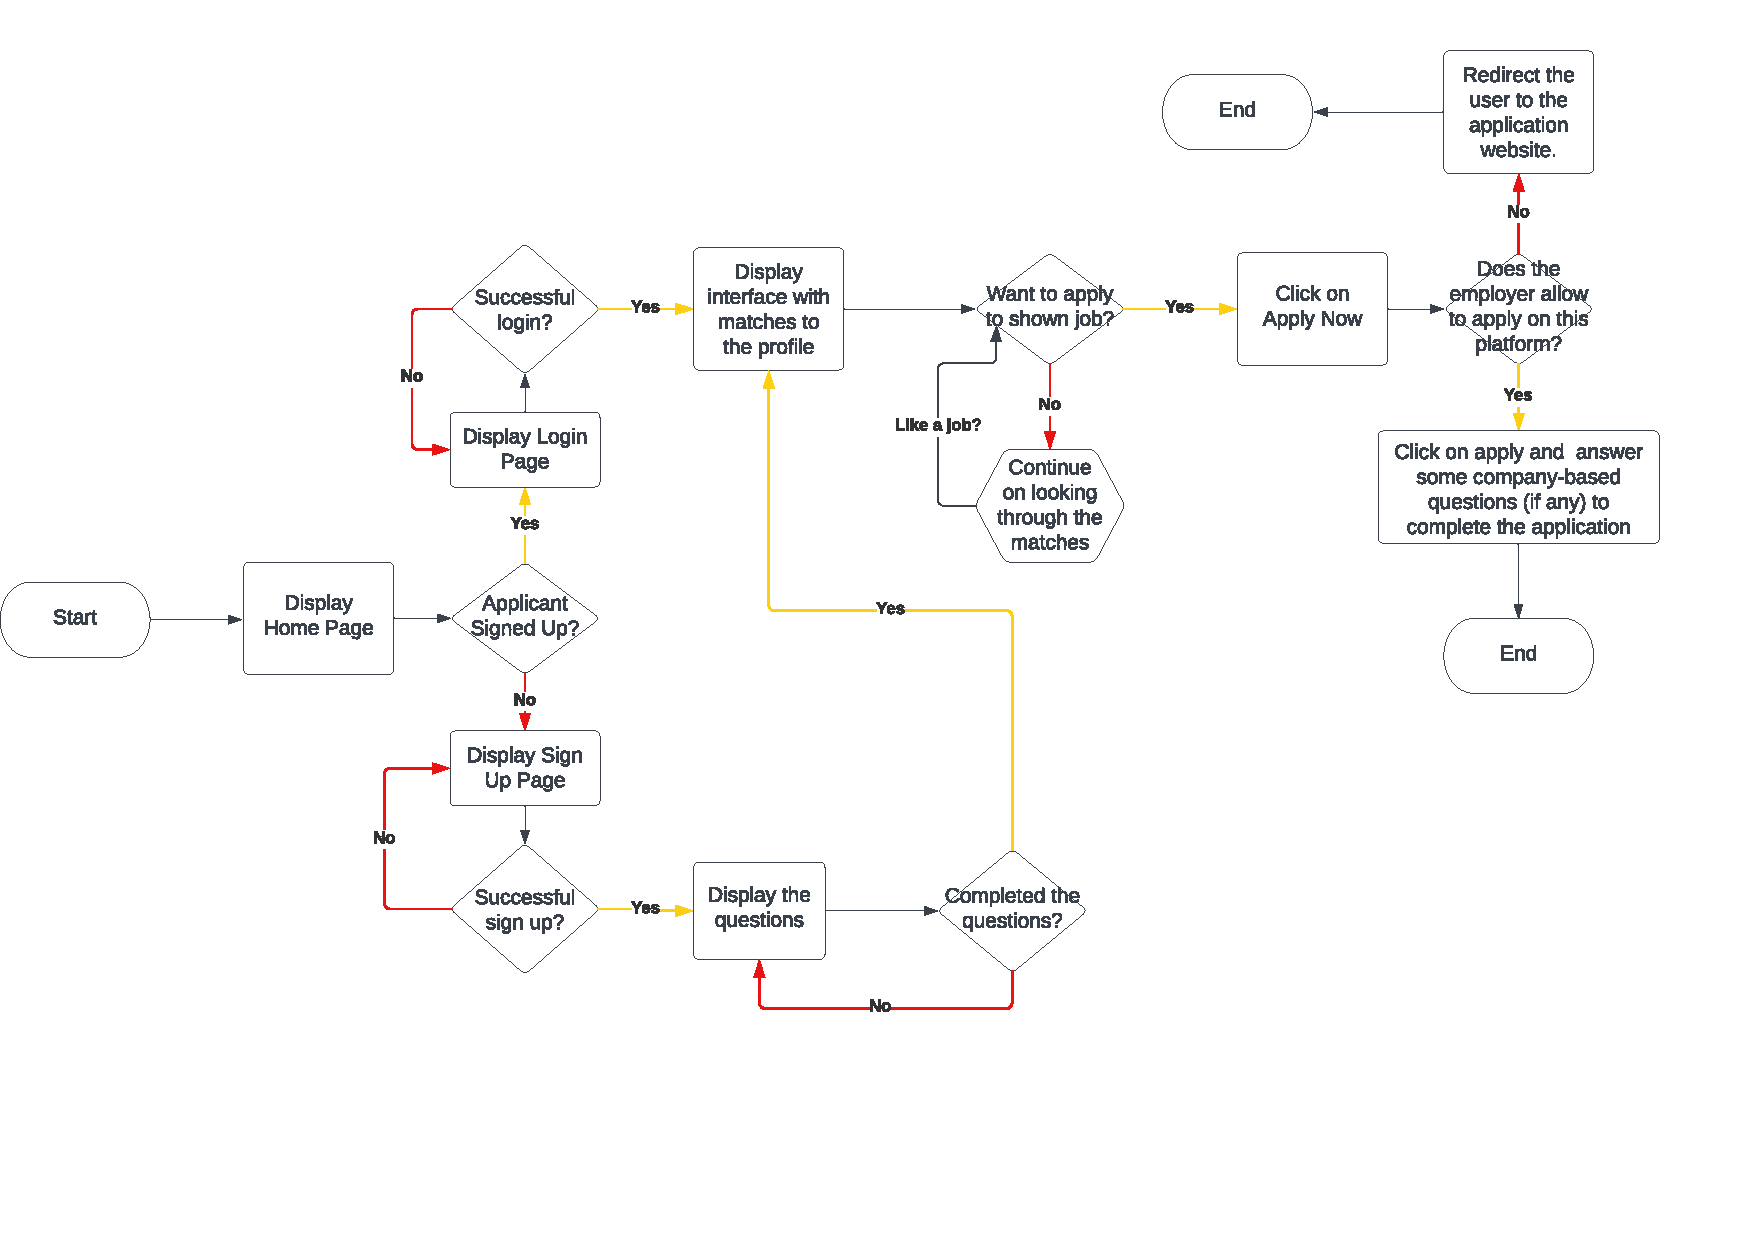
\includegraphics[width = 140mm]{Figures/applying.pdf}
    \decoRule
    \caption[Use Case Diagram for applying for a job]{Use Case Diagram for applying for a job}
    \label{fig: Use Case Diagram for applying for a job}
\end{figure}

\begin{figure}
    \noindent
    \centering
    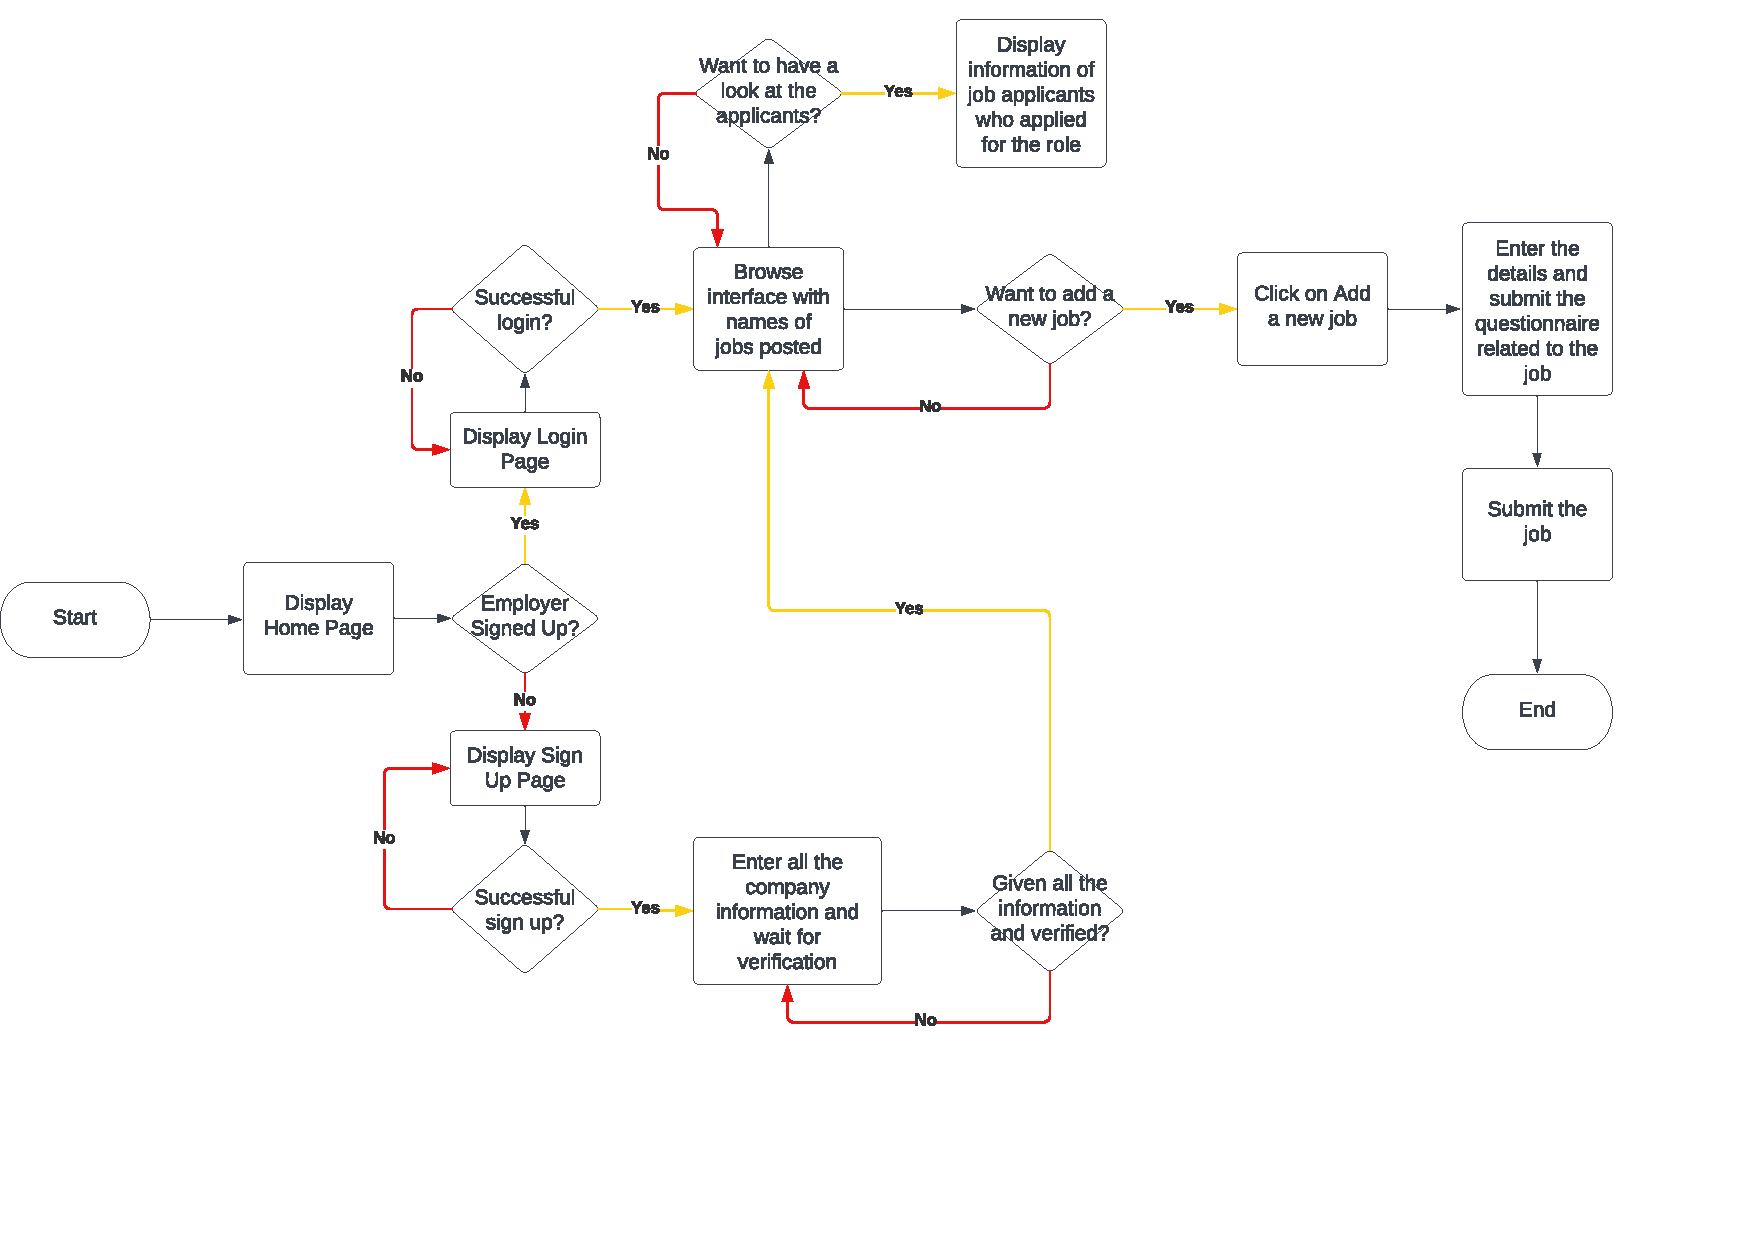
\includegraphics[width = 140mm]{Figures/employer.pdf}
    \decoRule
    \caption[Use Case Diagram for an Employer to add a new job]{Use Case Diagram for an Employer to add a new job}
    \label{fig: Use Case Diagram for an Employer to add a new job}
\end{figure}

\newpage
\subsection{Designs}
Some wireframes and designs were created to help visualise what specific pages will look like. This is the first prototype of these designs, which can be changed in the future based on user feedback. The goal of these is to create a simple design. 

The home screen shown in figure \ref{fig: Home Screen} shows the links on the header where applicants can click login to be redirected to the login page shown in figure \ref{fig: Login Page}. The home page still needs improvement, as some links aren't positioned where they should be, and some placeholder text is used in places. 

As shown in figure \ref{fig: Job Posting}, the job details are given on the right-hand side, and the company details are provided on the left-hand side. This helps users know which side to look for each component. Also, each section has a heading to make it even easier to find the details the applicant is looking for. The user can click on arrows on the right side to look at the next role or click on the arrow back to look at the previous job. If applicants want to apply, they can click on the apply button. Some design changes are needed on this page as the apply button isn't centred enough and doesn't seem appealing.

\begin{figure}
    \noindent
    \centering
    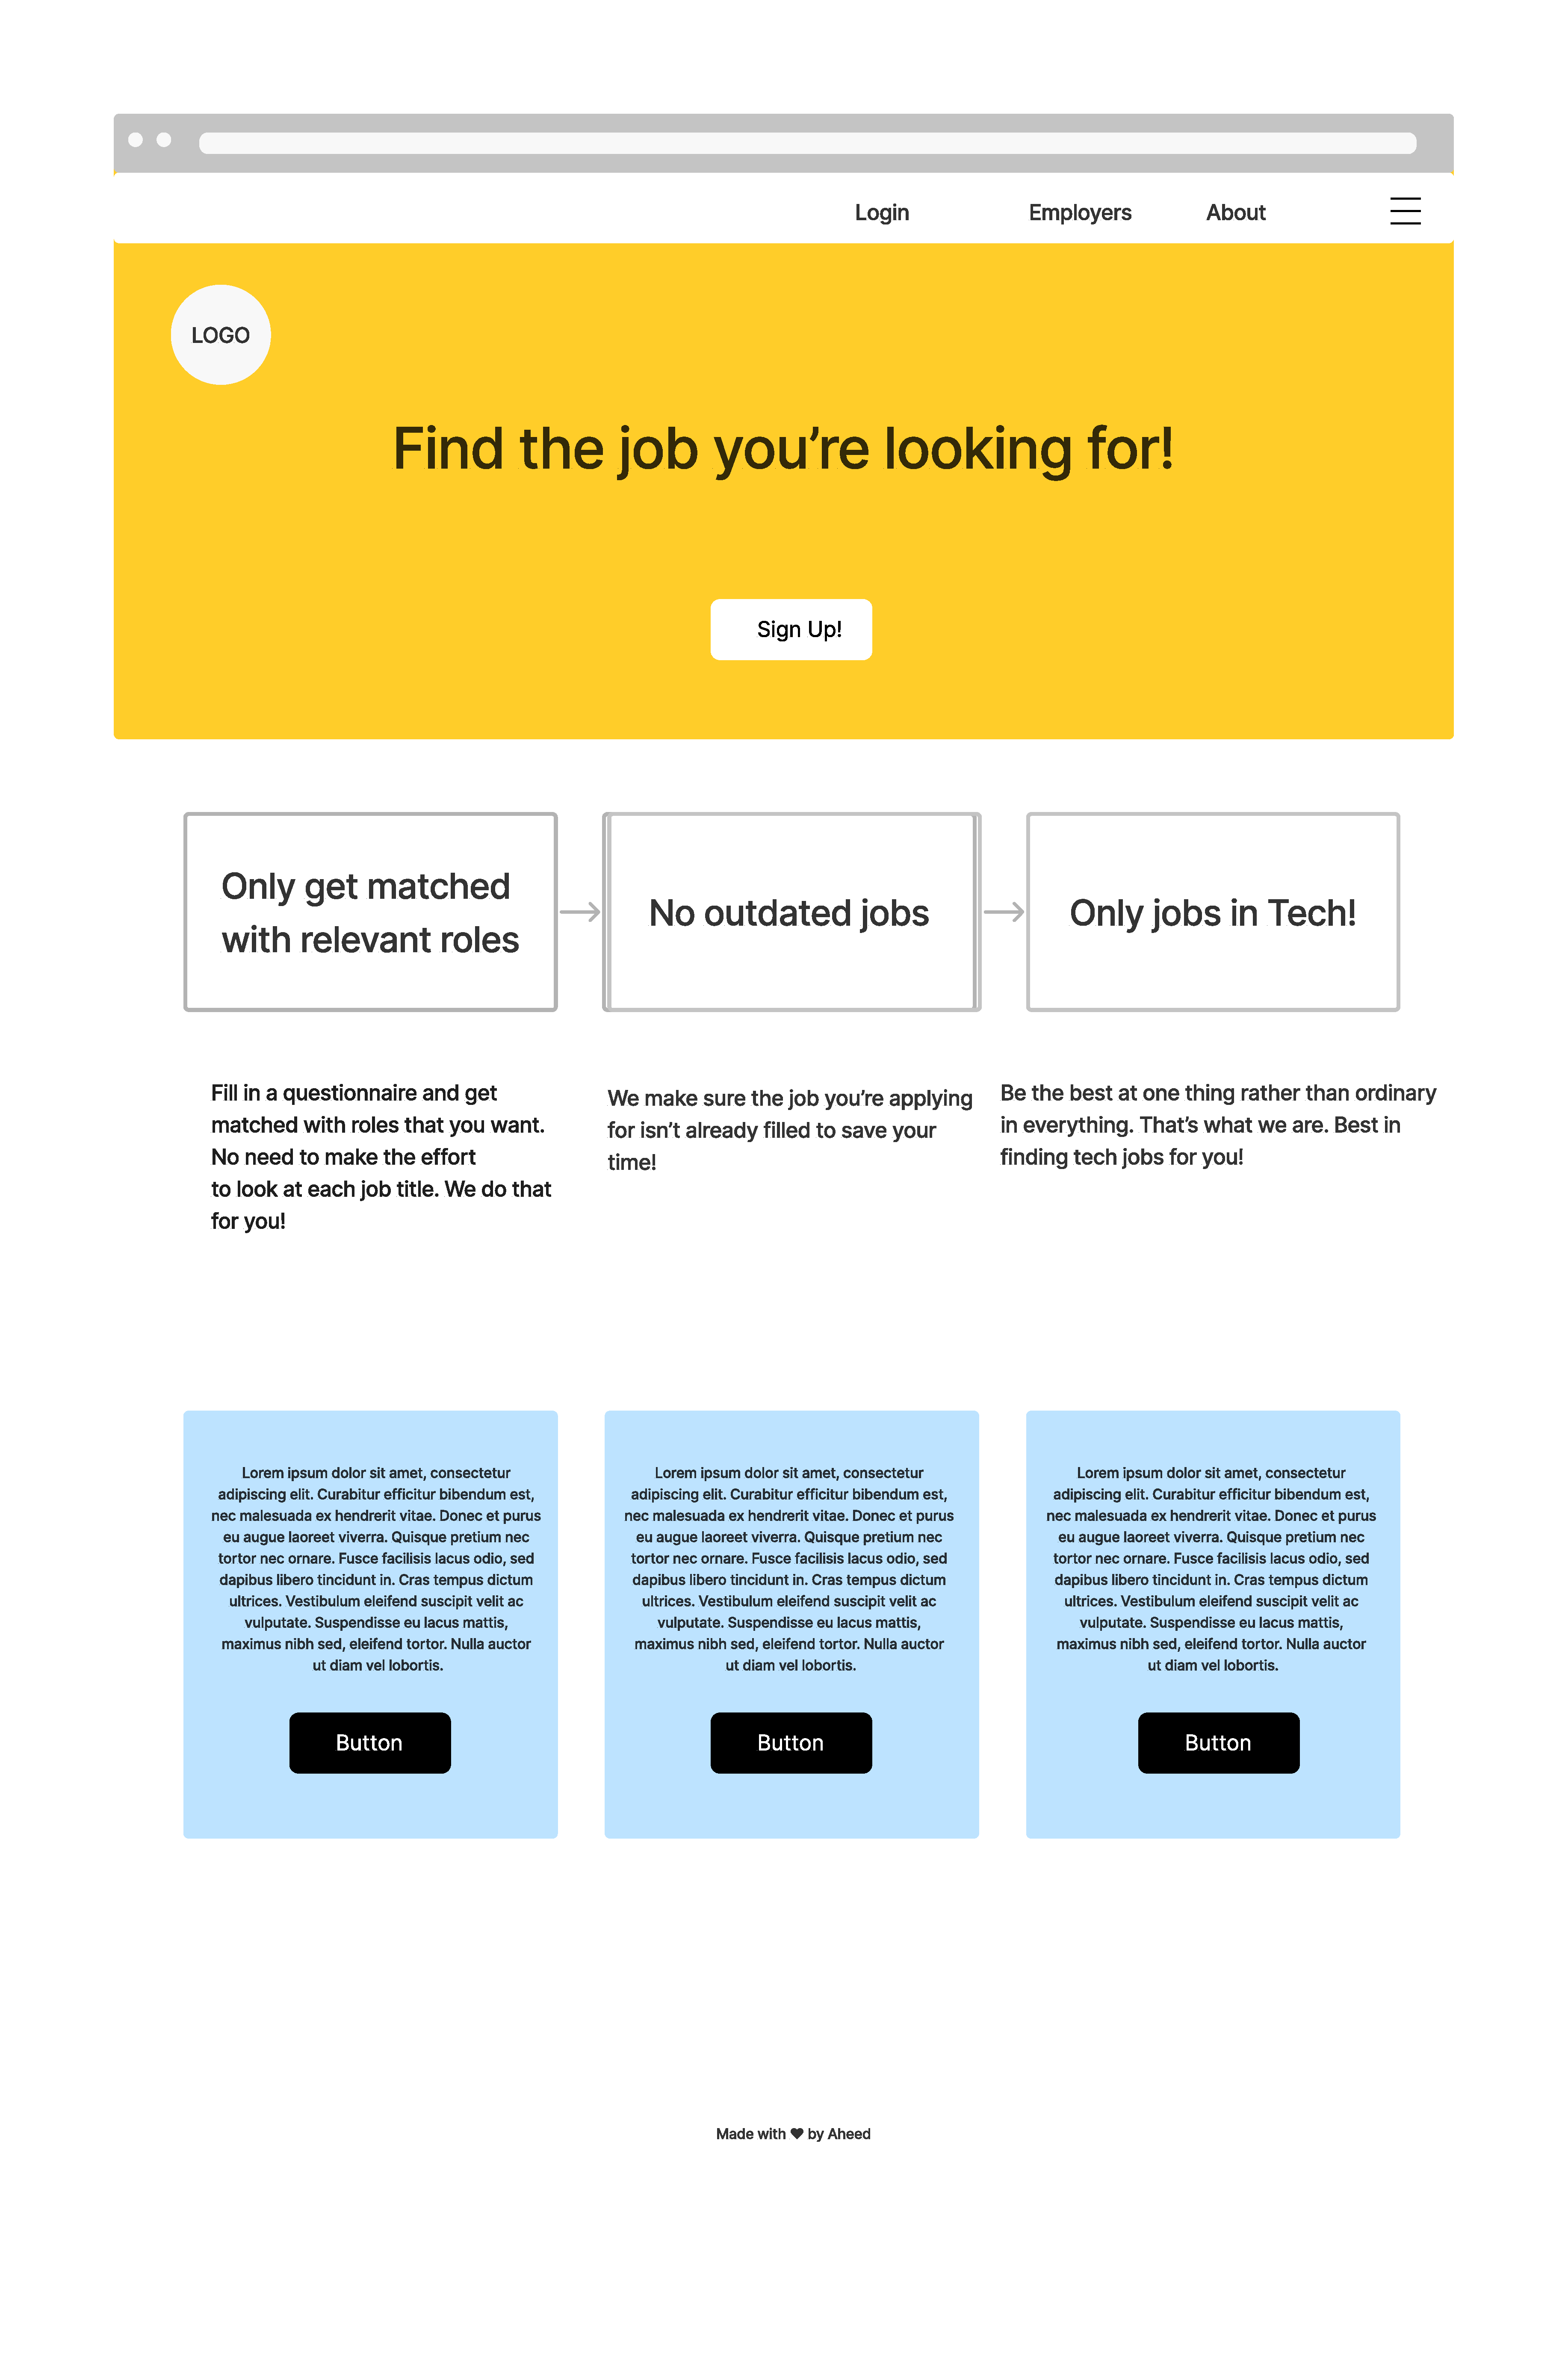
\includegraphics[width = 140mm]{Figures/homescreen.pdf}
    \decoRule
    \caption[Home Screen of the application]{Home Screen of the application}
    \label{fig: Home Screen}
\end{figure}

\begin{figure}
    \noindent
    \centering
    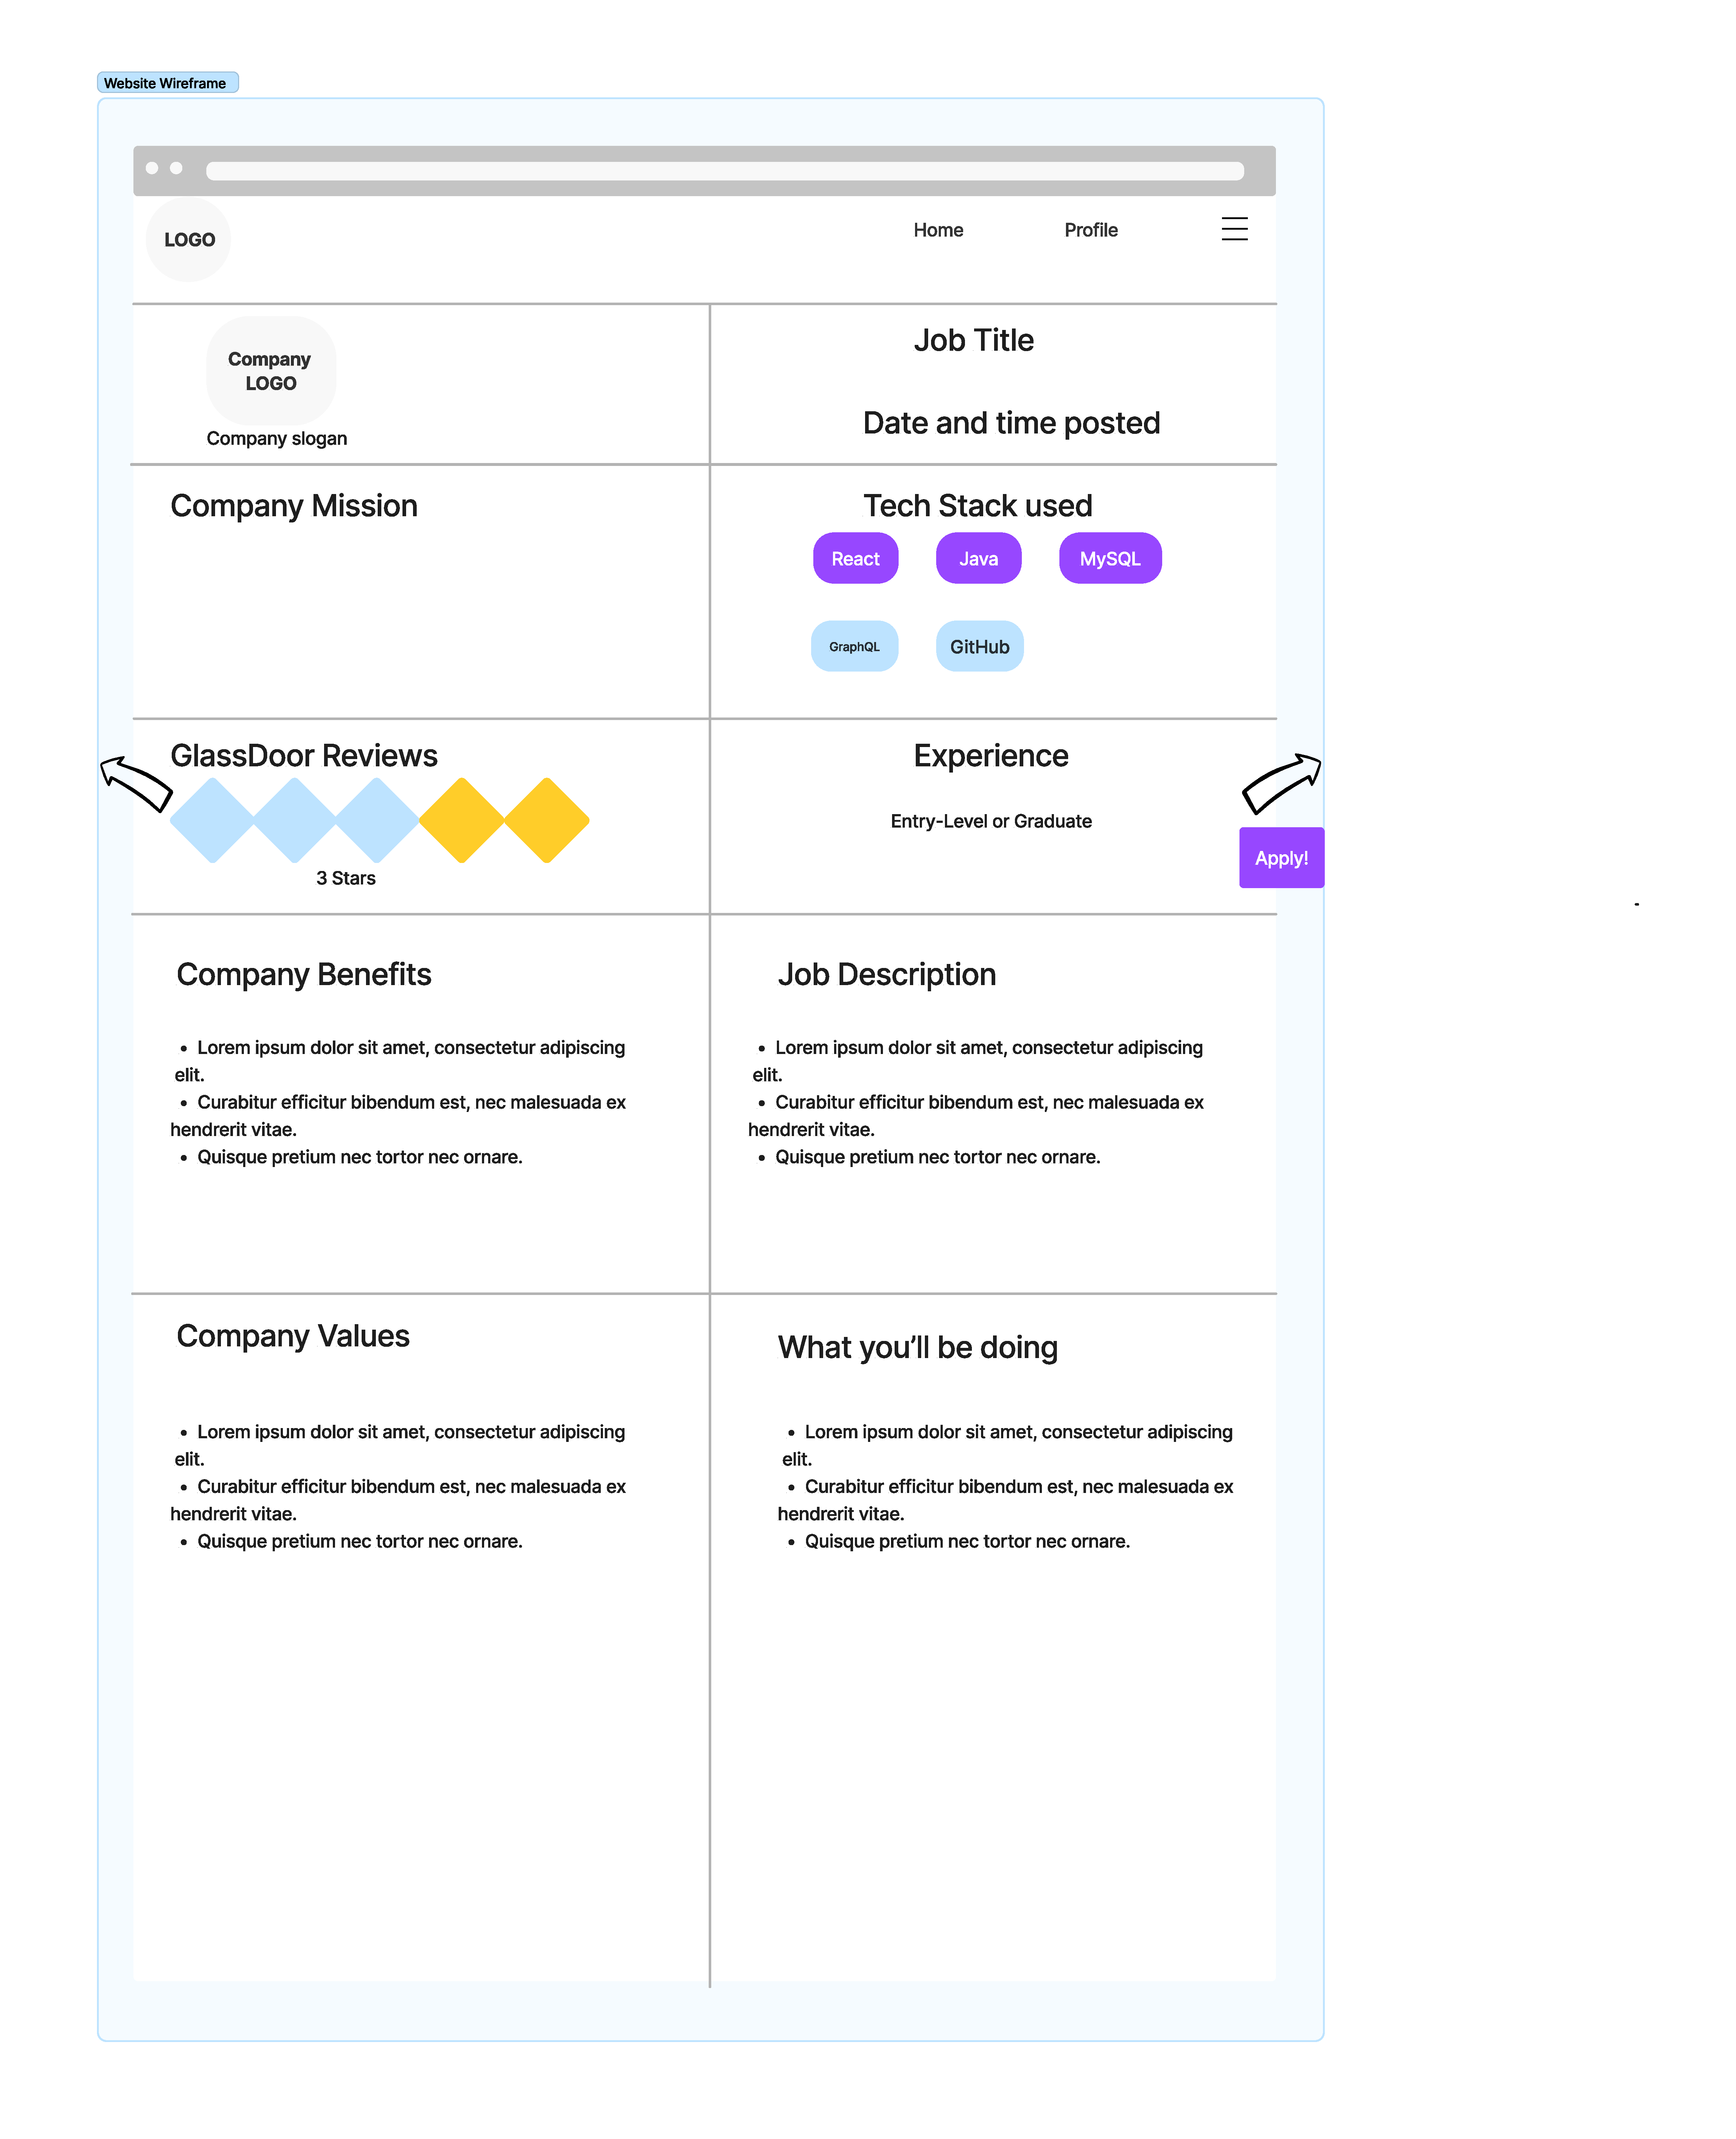
\includegraphics[width = 140mm]{Figures/posting.pdf}
    \decoRule
    \caption[Example of a job posting on the application]{Example of a job posting on the application}
    \label{fig: Job Posting}
\end{figure}

\begin{figure}
    \noindent
    \centering
    \includegraphics[width = 140mm]{Figures/loginPage.pdf}
    \decoRule
    \caption[Login Page]{Login Page}
    \label{fig: Login Page}
\end{figure}


\newpage
\section{Future Work}
While the first prototype of the designs is ready, they are not user-tested. These designs will be given to different users to provide feedback which will be noted and implemented in the future during the implementation of this application. 

As the implementation of this application is ongoing, multiple iterations will be done in the design, and as a result, the application's design will continue to change. Some things noted in the previous sections will also be worked on in the coming months, such as having similar colour choices throughout the application to make it more user-friendly. 

Testing is also one of the critical things that must be done in the Implementation stage. User Testing, Unit Testing, and Integration Testing are some tests which will be done in the implementation stage. 

Hosting the application will be done on the University Servers, and users will be able to provide feedback on the application by using it on their devices. This will prove beneficial as different devices using different browsers may have some errors which could be fixed during the implementation stage. 

In the MVP of this application, an employer should be able to add and create a new job posting, which the applicant should be able to see if their requirements meet the employers. All functional requirements should also be met for the MVP of this application.